\chapter{Implementation}
\label{ch:implementation}

Chapter~\ref{ch:ivm} described the IVM$^+$ approach and its variant at the level of relational algebra, independently of any particular engine.
This chapter realises them on Feldera and presents the two tools we built: a \emph{query decomposer} and an \emph{experiment harness}.

The two share a single artifact, the set of \emph{SQL views} that encode a decomposition.
The query decomposer produces these views from an input query, and the experiment harness deploys them as a Feldera pipeline, runs it over the input data, and measures performance.
Figure~\ref{fig:ch4_overview} shows the two components.

The SQL views used in our evaluation were written by hand rather than produced by the decomposer, which we developed afterwards to generate them automatically.
They are semantically equivalent to its output and differ only in syntax.

\begin{figure}[ht]
  \centering
  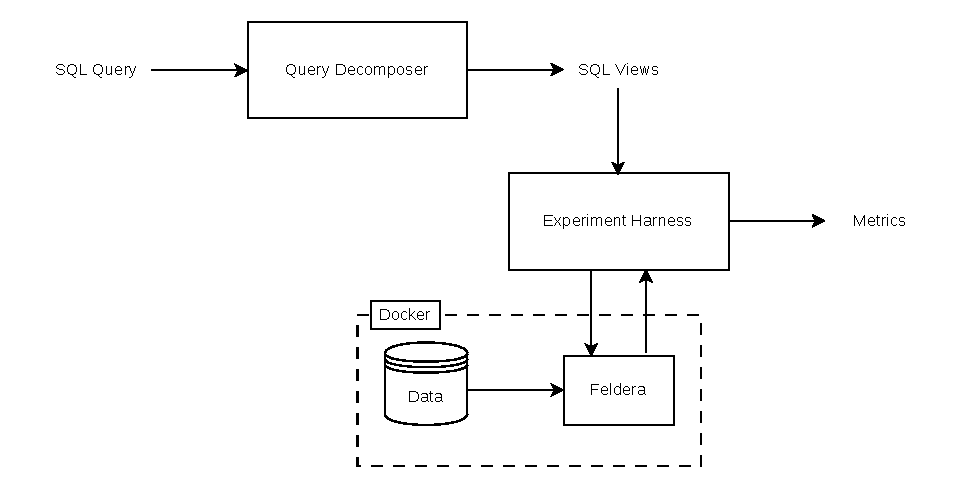
\includegraphics[width=\textwidth]{./figures/ch4_overview.pdf}
  \caption{Overview of the query decomposer and the experiment harness.}
  \label{fig:ch4_overview}
\end{figure}

We first give the necessary background on how Feldera works, then show how the decomposition of Chapter~\ref{ch:ivm} becomes a Feldera pipeline, and finally describe the decomposer and the harness in turn.

\section{Feldera}
\label{sec:feldera}

Feldera is a query engine for \emph{incremental computation}~\cite{feldera2026}.
A computation is expressed in SQL, and Feldera maintains its results as the input data changes, updating them from the changes alone rather than recomputing over all the data.
This incremental evaluation is founded on the DBSP model~\cite{budiu2023DBSP} and applies to arbitrary SQL queries.

A Feldera \emph{pipeline} is a set of SQL tables and views~\cite{feldera2026}.
The tables are the inputs, and the views are derived from them and can be nested within one another.
As changes arrive at the tables, Feldera updates every view accordingly.
This maps directly onto the construction of Chapter~\ref{ch:ivm}: the bag relations become SQL views, defined bottom-up from the base tables and the child bags' views, so the IVM$^+$ approach and its variant run as an ordinary Feldera pipeline on an unmodified engine.

Changes reach a pipeline's tables in three ways: through \emph{input connectors} attached to the tables, through HTTP requests, or through ad-hoc \texttt{INSERT} statements~\cite{feldera2026}.
Our experiments use input connectors, which read the input data from CSV files.
We chose them over HTTP ingress, which in our tests was slow enough to make ingestion, rather than the incremental computation, the bottleneck.

By default, Feldera stores only the data needed to compute future outputs, not the complete contents of every table and view~\cite{feldera2026}.
A table or view can be declared \emph{materialized} to keep its full contents available, for example to inspect or query them directly.
A table with a \texttt{PRIMARY KEY} is materialized automatically, since Feldera must maintain a key index.
Materializing a table or view can slow the pipeline down, as more data must be written to storage, which can also increase the pipeline's memory use.

\section{Decomposition as a Feldera Pipeline}
\label{sec:pipeline}

This section realises the construction of Chapter~\ref{ch:ivm} as a Feldera pipeline.
Each bag becomes a \emph{$Q'$-view} for its $Q'$-relation and a \emph{$P'$-view} for its $P'$-relation.
The views are built bottom-up, so a child's $P'$-view is ready when its parent's $Q'$-view is computed, and a final \texttt{RESULT} view produces the query's output.
We name a non-root bag's views \texttt{BAG\_N\_QPRIME} and \texttt{BAG\_N\_PPRIME}, and the root's \texttt{ROOT\_QPRIME}.
IVM$^+$ and the variant differ only in how the $Q'$-view is defined.
The view definitions are ordinary SQL, and only the input connectors and the materialisation annotations on the tables are specific to Feldera.

\subsection{Tables and connectors}

The base tables carry a Feldera \emph{input connector} that specifies where the pipeline reads its data.
For $Q_\diamond$, whose five atoms are all occurrences of one edge relation, this is a single table \texttt{EDGES(src, tgt)} with a connector that reads a CSV file:

\begin{lstlisting}[caption={The \texttt{EDGES} table with a CSV input connector.}]
CREATE TABLE EDGES (
    src BIGINT,
    tgt BIGINT
) WITH (
    'materialized' = 'true',
    'connectors' = '[{
        "transport": {
            "name": "file_input",
            "config": { 
                "path": "edges.csv" 
                } 
        },
        "format": { 
            "name": "csv", 
            "config": { 
                "headers": true 
            } 
        }
    }]'
);
\end{lstlisting}

Besides the connector, the table is declared \texttt{'materialized'}, the annotation from Section~\ref{sec:feldera} that keeps its full contents available.
The connector and this annotation are the only Feldera-specific parts of the declaration.
The views built on the table, described next, are ordinary SQL.

\subsection{Bag views}

A bag's \emph{$P'$-view} projects its \emph{$Q'$-view} onto the bridge variables, giving the set of bridge values with which the parent filters its own tuples (Chapter~\ref{ch:ivm}).
Here SQL's bag semantics matter: a plain projection keeps duplicate rows, but the $P'$-relation must be a \emph{set}, or the duplicates would multiply the parent's tuples when it joins with the view.
We therefore use \texttt{SELECT DISTINCT}.
For $Q_\diamond$, the child bag $b_2 = \{B,C,D\}$ shares $\{B,D\}$ with the root, so its $P'$-view is:

\begin{lstlisting}[caption={The $P'$-view of the child bag $b_2$.}]
CREATE MATERIALIZED VIEW BAG_2_PPRIME AS
SELECT DISTINCT B, D
FROM BAG_2_QPRIME;
\end{lstlisting}

The view is materialized and can therefore be queried directly (Section~\ref{sec:feldera}).
The $Q'$-view \texttt{BAG\_2\_QPRIME} it reads from is defined next.

We define a bag's $Q'$-view by joining its atoms on their shared variables with \texttt{USING}.
Unlike an \texttt{ON} join, \texttt{USING} merges each pair of shared columns into one, so \texttt{SELECT *} returns exactly the bag's variables and the views chain cleanly.
Because $Q_\diamond$ is a self-join, with every atom an occurrence of the same \texttt{EDGES} relation, each atom is written as a subquery that renames \texttt{src} and \texttt{tgt} to that atom's variables.
For IVM$^+$, a partially overlapping atom is added as an inline \texttt{SELECT DISTINCT} semijoin.
The child bag $b_2$ is a leaf, so its $Q'$-view is just its atoms:

\begin{lstlisting}[caption={The $Q'$-view of the child bag $b_2$ (IVM$^+$).}]
CREATE MATERIALIZED VIEW BAG_2_QPRIME AS
SELECT *
FROM (SELECT src AS B, tgt AS C FROM EDGES)
JOIN (SELECT src AS C, tgt AS D FROM EDGES) USING (C)
JOIN (SELECT src AS B, tgt AS D FROM EDGES) USING (B, D)
JOIN (SELECT DISTINCT tgt AS B FROM EDGES) USING (B)
JOIN (SELECT DISTINCT tgt AS D FROM EDGES) USING (D);
\end{lstlisting}

The first three subqueries are the contained atoms $E_2(B,C)$, $E_3(C,D)$, and $E_4(B,D)$, joined on their shared variables.
The last two are the semijoins $\pi_B E_1$ and $\pi_D E_5$, restricting $B$ and $D$ to values that occur in those atoms.
The variant keeps only the fully contained atoms and drops the two semijoins:

\begin{lstlisting}[caption={The $Q'$-view of the child bag $b_2$ (variant).}]
CREATE MATERIALIZED VIEW BAG_2_QPRIME AS
SELECT *
FROM (SELECT src AS B, tgt AS C FROM EDGES)
JOIN (SELECT src AS C, tgt AS D FROM EDGES) USING (C)
JOIN (SELECT src AS B, tgt AS D FROM EDGES) USING (B, D);
\end{lstlisting}

A non-leaf bag is built the same way but also joins its children's $P'$-views on the bridge variables.
The root's $Q'$-view \texttt{ROOT\_QPRIME}, for example, joins \texttt{BAG\_2\_PPRIME} using $\{B,D\}$.

\subsection{Result reconstruction}

The full query result is reconstructed by joining all the $Q'$-views on their shared variables (Chapter~\ref{ch:ivm}).
For $Q_\diamond$ this is a single join of the root and child $Q'$-views on the bridge variables $\{B,D\}$:

\begin{lstlisting}[caption={The \texttt{RESULT} view reconstructing the full output.}]
CREATE MATERIALIZED VIEW RESULT AS
SELECT *
FROM ROOT_QPRIME
JOIN BAG_2_QPRIME USING (B, D);
\end{lstlisting}

This \texttt{RESULT} view is the terminal view an experiment measures.
We also consider a variant \emph{without reconstruction} that omits this final join: the root's $Q'$-view \texttt{ROOT\_QPRIME} is the terminal view instead.
This isolates the cost of maintaining the bag views from the cost of joining them back into the full result.
For aggregate queries the terminal view is neither of these, but the aggregate itself, computed as described next.

\subsection{Computing \texttt{COUNT(*)}}

The number of result tuples returned by \texttt{COUNT(*)} can be computed directly on the decomposition, without materialising the full result (Section~\ref{sec:semiring}).
Each $P'$-view then carries a \emph{count} beside its bridge variables: instead of \texttt{SELECT DISTINCT}, it groups by the bridge variables and records how many tuples fall in each group.
A leaf bag's count is \texttt{COUNT(*)}: every tuple has an implicit count of one, so counting the rows in each group gives its count, with no explicit sum.
A bag with children instead multiplies its children's counts and sums the products within each group.
For $Q_\diamond$, the child bag $b_2$ is a leaf, so its $P'$-view groups by $\{B,D\}$ and counts:

\begin{lstlisting}[caption={The $P'$-view of the child bag, carrying a count.}]
CREATE MATERIALIZED VIEW BAG_2_PPRIME AS
SELECT B, D, COUNT(*) AS ANNOTATION_2
FROM BAG_2_QPRIME
GROUP BY B, D;
\end{lstlisting}

The root's $Q'$-view joins this $P'$-view as before, and so carries the column \texttt{ANNOTATION\_2}.
The \texttt{RESULT} view is then the sum over the root's $Q'$-view of the counts contributed by its child:

\begin{lstlisting}[caption={The \texttt{RESULT} view computing \texttt{COUNT(*)}.}]
CREATE MATERIALIZED VIEW RESULT AS
SELECT SUM(ANNOTATION_2) AS RESULT
FROM ROOT_QPRIME;
\end{lstlisting}

This \texttt{RESULT} is the number of tuples in the result of $Q_\diamond$, which is its \texttt{COUNT(*)}.
Because every input tuple has an implicit annotation of one, the base tables need no annotation column, and an atom appearing in several bags is not double-counted, since multiplying by one changes nothing.
An aggregate that reads a column, such as \texttt{MIN}, has no such implicit annotation: each relation must then carry its value explicitly and be counted in a single \emph{canonical} bag, or its value would be combined more than once.
We therefore implement only \texttt{COUNT(*)}.

\section{Query Decomposer}
\label{sec:decomposer}

Section~\ref{sec:pipeline} built the SQL views for $Q_\diamond$ by hand.
The \emph{query decomposer} automates this: given a query, it computes a tree decomposition and emits the corresponding $Q'$- and $P'$-views, in both the IVM$^+$ and the variant form.
It is the tool one would run to obtain a pipeline for a new query, without working through the decomposition by hand.

The decomposer takes two inputs, the query and the schema of the tables it refers to, and returns the set of SQL views.
It proceeds in four stages, shown in Figure~\ref{fig:decomposer}: a \emph{parser} reads the SQL, a \emph{hypergraph} is built from the query, a tree \emph{decomposition} is computed over it, and a \emph{generator} emits the views.
We describe each stage in turn.

\begin{figure}[ht]
  \centering
  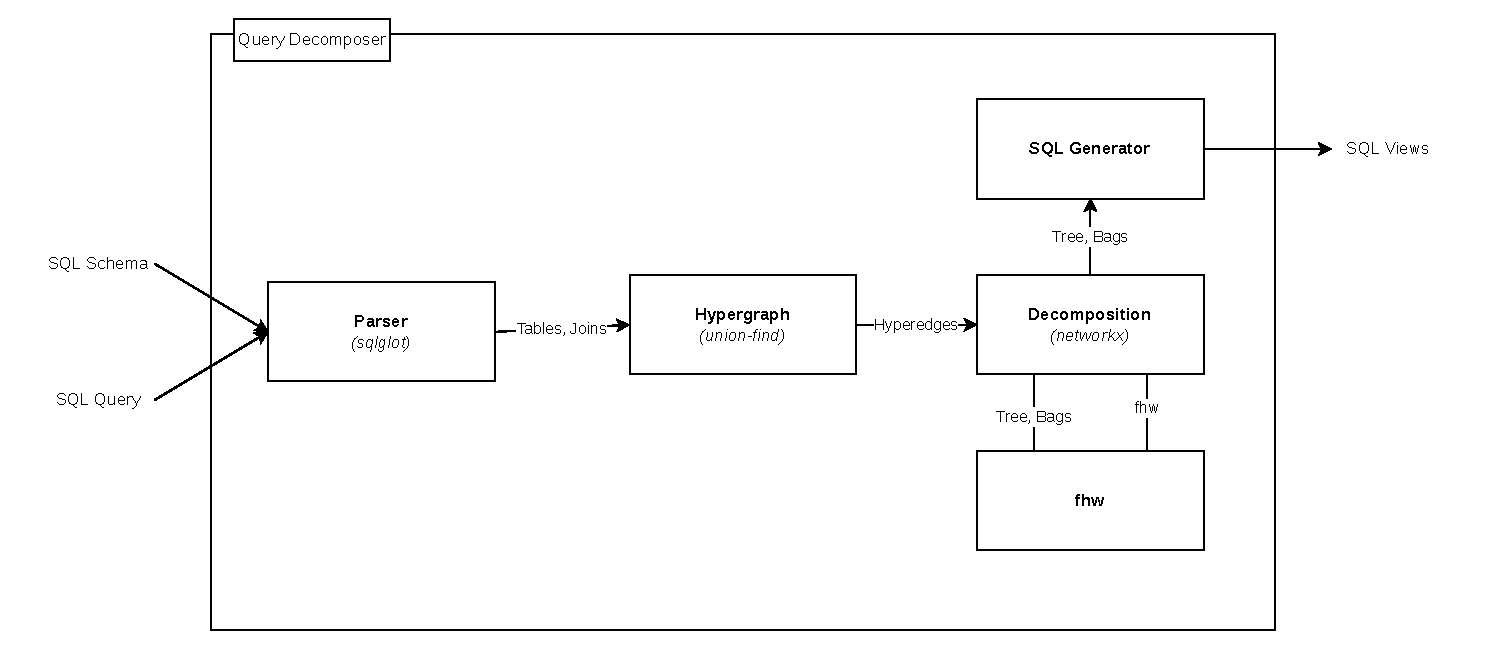
\includegraphics[width=\textwidth]{./figures/ch4_query_decomposer.pdf}
  \caption{The stages of the query decomposer.}
  \label{fig:decomposer}
\end{figure}

\subsection{Parser}

The parser reads the two SQL inputs, the schema and the query, and extracts the structure the later stages work on.
It needs the full schema, not just the query, for two reasons.
First, the tool returns the full conjunctive query, so it must know every attribute of every relation, including those the query never mentions.
Second, the hypergraph has one vertex per variable, so all variables must be known even where the query does not reference them.
Parsing itself uses \emph{sqlglot}, which turns the SQL into an abstract syntax tree that we then traverse.

The parser traverses the syntax tree clause by clause.
It first reads the \texttt{SELECT} clause, which fixes whether the query asks for the full result or a \texttt{COUNT(*)}.
It then walks the \texttt{FROM} clause and each \texttt{JOIN} clause in turn, and as it reaches a table it registers it, resolving its alias and recording its variables.
SQL lets a query rename tables and columns and use the same relation more than once, so a self-join, where one relation appears under several aliases, is registered as several independent relations, matching the atoms of Section~\ref{sec:queries}: the five occurrences of \texttt{EDGES} in $Q_\diamond$ become five relations $E_1,\dots,E_5$.
In the same pass it reads each join's equi-join condition, written as \texttt{JOIN \ldots ON} or \texttt{JOIN \ldots USING}, telling the next stage which columns are equated and therefore collapse into a single vertex of the hypergraph, even where those columns have different names.
Finally it reads the \texttt{WHERE} clause, collecting any single-relation filters.
The relations, their variables, the join conditions, and the single-relation filters are then passed on to the later stages.
The queries the parser accepts, and what it rejects, are set out in Section~\ref{sec:decomposer_limits}.

\subsection{Hypergraph}

The hypergraph stage builds the query's hypergraph, defined in Section~\ref{sec:tree_decompositions}: its vertices are the query's variables and each relation contributes one hyperedge.
A \emph{column} is an attribute of a relation in the SQL text, while a \emph{variable} is a vertex of the hypergraph, and a single variable can stand for several columns.
As noted above, an equi-join can equate two columns that do not share a name, and equated columns denote the same variable, so they must collapse into one.
The stage computes this with a \emph{union-find} structure: every column starts in its own group, each join condition merges the groups of the two columns it equates, and each final group is one variable.
Merging groups rather than pairs handles chains of joins, where equating $A=B$ and $B=C$ places all three columns in one variable.
Each variable takes its name from one of its columns, so two different variables would clash when their columns happen to share a name although no join equates them.
The stage renames such variables to keep every name distinct.
It also records, in both directions, which column of each relation a variable stands for, since the generator later needs to recover the physical column behind each variable.
Each relation then contributes one hyperedge, the set of variables of its columns.
For $Q_\diamond$ this yields the four variables $A,B,C,D$ and five hyperedges, the diamond of Figure~\ref{fig:diamond_hypergraph}, which is passed to the decomposition stage.

\subsection{Decomposition}

Section~\ref{sec:fhw} noted that computing a tree decomposition of minimum fractional hypertree width is NP-hard, so the decomposer uses a heuristic instead.
It relies on the Minimum Fill-in heuristic from the \emph{networkx} library, which operates on ordinary graphs rather than hypergraphs, so the stage first builds the \emph{primal graph} of the hypergraph: each hyperedge, that is each relation's set of variables, becomes a clique.
Making every hyperedge a clique forces its variables into a common bag, so a tree decomposition of the primal graph is a tree decomposition of the hypergraph~\cite{grohe2014}.

Minimum Fill-in is a vertex-elimination heuristic for finding a decomposition of small treewidth~\cite{bodlaender2005}.
It repeatedly eliminates the vertex whose neighbourhood is closest to a clique, measured by its number of \emph{fill-in edges}, the edges missing among its neighbours that would make them pairwise adjacent.
A vertex whose neighbours are already pairwise adjacent has no fill-in.
To eliminate a vertex the heuristic adds those missing edges, making its neighbours a clique, records the vertex together with its neighbours as a bag, and removes the vertex and its incident edges.
From these bags networkx forms the tree.
The stage then removes any bag contained in a neighbouring bag, so that none is redundant.

A single run of Minimum Fill-in produces one decomposition.
When several vertices tie for the fewest fill-in edges, the networkx implementation breaks the tie by the order in which the vertices were inserted into the primal graph.
The decomposer exploits this to obtain several candidates: it runs Minimum Fill-in once for each of a number of insertion orderings, a sorted baseline and twenty seeded shuffles, so that different tie-breaks yield different decompositions.

Minimum Fill-in targets small treewidth, but the IVM$^+$ approach wants small fractional hypertree width (Section~\ref{sec:fhw}).
The two are related: the fractional hypertree width of a query is at most its treewidth plus one~\cite{grohe2014}, so decompositions of small treewidth are a good source of ones of small fractional hypertree width.
But two decompositions of equal treewidth can still differ in fractional hypertree width, so the decomposer computes it for each candidate and keeps the smallest, breaking ties by treewidth.
The fractional hypertree width of a candidate is the largest fractional edge cover number over its bags, obtained by solving the linear program of Section~\ref{sec:fhw} with \emph{scipy}.
For $Q_\diamond$ this selects the two-triangle decomposition of Figure~\ref{fig:diamond_td}, of fractional hypertree width $\tfrac{3}{2}$.
The selected bags and tree are passed to the SQL generator.

\subsection{SQL generator}

The generator turns the bags and tree from the previous stage into the SQL views of Section~\ref{sec:pipeline}, producing automatically the translation presented there for $Q_\diamond$.
It first \emph{orients} the tree by choosing a root, by default bag~1, though any bag may serve as root, which gives every bag a parent and a set of children.
For each non-root bag it then computes the \emph{bridge variables} it shares with its parent.

The views are emitted bottom-up, each bag after its children, so a child's $P'$-view is ready when its parent needs it, matching the construction of Section~\ref{sec:pipeline}.
For a bag, the generator builds its $Q'$-view from the atoms.
Each atom becomes a subquery over its underlying table: using the mapping the hypergraph stage recorded, the generator selects the physical column each of the bag's variables stands for and aliases it to the variable, as in the \texttt{src AS B} of Section~\ref{sec:pipeline}, and appends the atom's single-relation filters as a \texttt{WHERE} clause.
The subqueries are joined with \texttt{JOIN \ldots USING} on their shared variables.
IVM$^+$ and the variant differ only here, in that IVM$^+$ adds a partially overlapping atom as a \texttt{SELECT DISTINCT} semijoin while the variant drops it (Section~\ref{sec:pipeline}).
The $Q'$-view is completed by joining the $P'$-views of the bag's children on the bridge variables, and the generator joins only on variables the view already contains, so it never references a column that is not there.
For a non-root bag it also emits the $P'$-view.

Finally the generator emits the \texttt{RESULT} view, the reconstruction join of all the $Q'$-views for a full-result query, or the single \texttt{COUNT(*)} scalar for an aggregate.
For $Q_\diamond$ the generator produces the views of Section~\ref{sec:pipeline}, up to the tool's own bag numbering.

The decomposer exposes two choices, each of which regenerates the views: switching between IVM$^+$ and the variant, and re-rooting the tree at a different bag.
Re-rooting changes the parent--child structure of the bags, and so the views and the size of the intermediate results they hold, even though the final result is unchanged.
How the orientation affects performance is examined in Chapter~\ref{ch:evaluation}, where we compare several orientations of the same query.

Figure~\ref{fig:decomposer_ui} shows the decomposer's web interface on $Q_\diamond$.
The schema and the query are entered at the top, on the left and right, and pressing \emph{Decompose} fills in the lower half.
On the left, the tree decomposition is drawn with each bag's number and variables and each edge's bridge variables, above a menu that selects the root.
On the right are the generated views, with a toggle between IVM$^+$ and the variant.
The interface labels the variant \texttt{IVM+*}~(strict), and the figure shows it, rooted at $\{A,B,D\}$ as in our example.
The tool assigns its own bag numbers, so the child bag $b_2$ appears here as \texttt{BAG\_1}.

\begin{figure}[H]
  \centering
  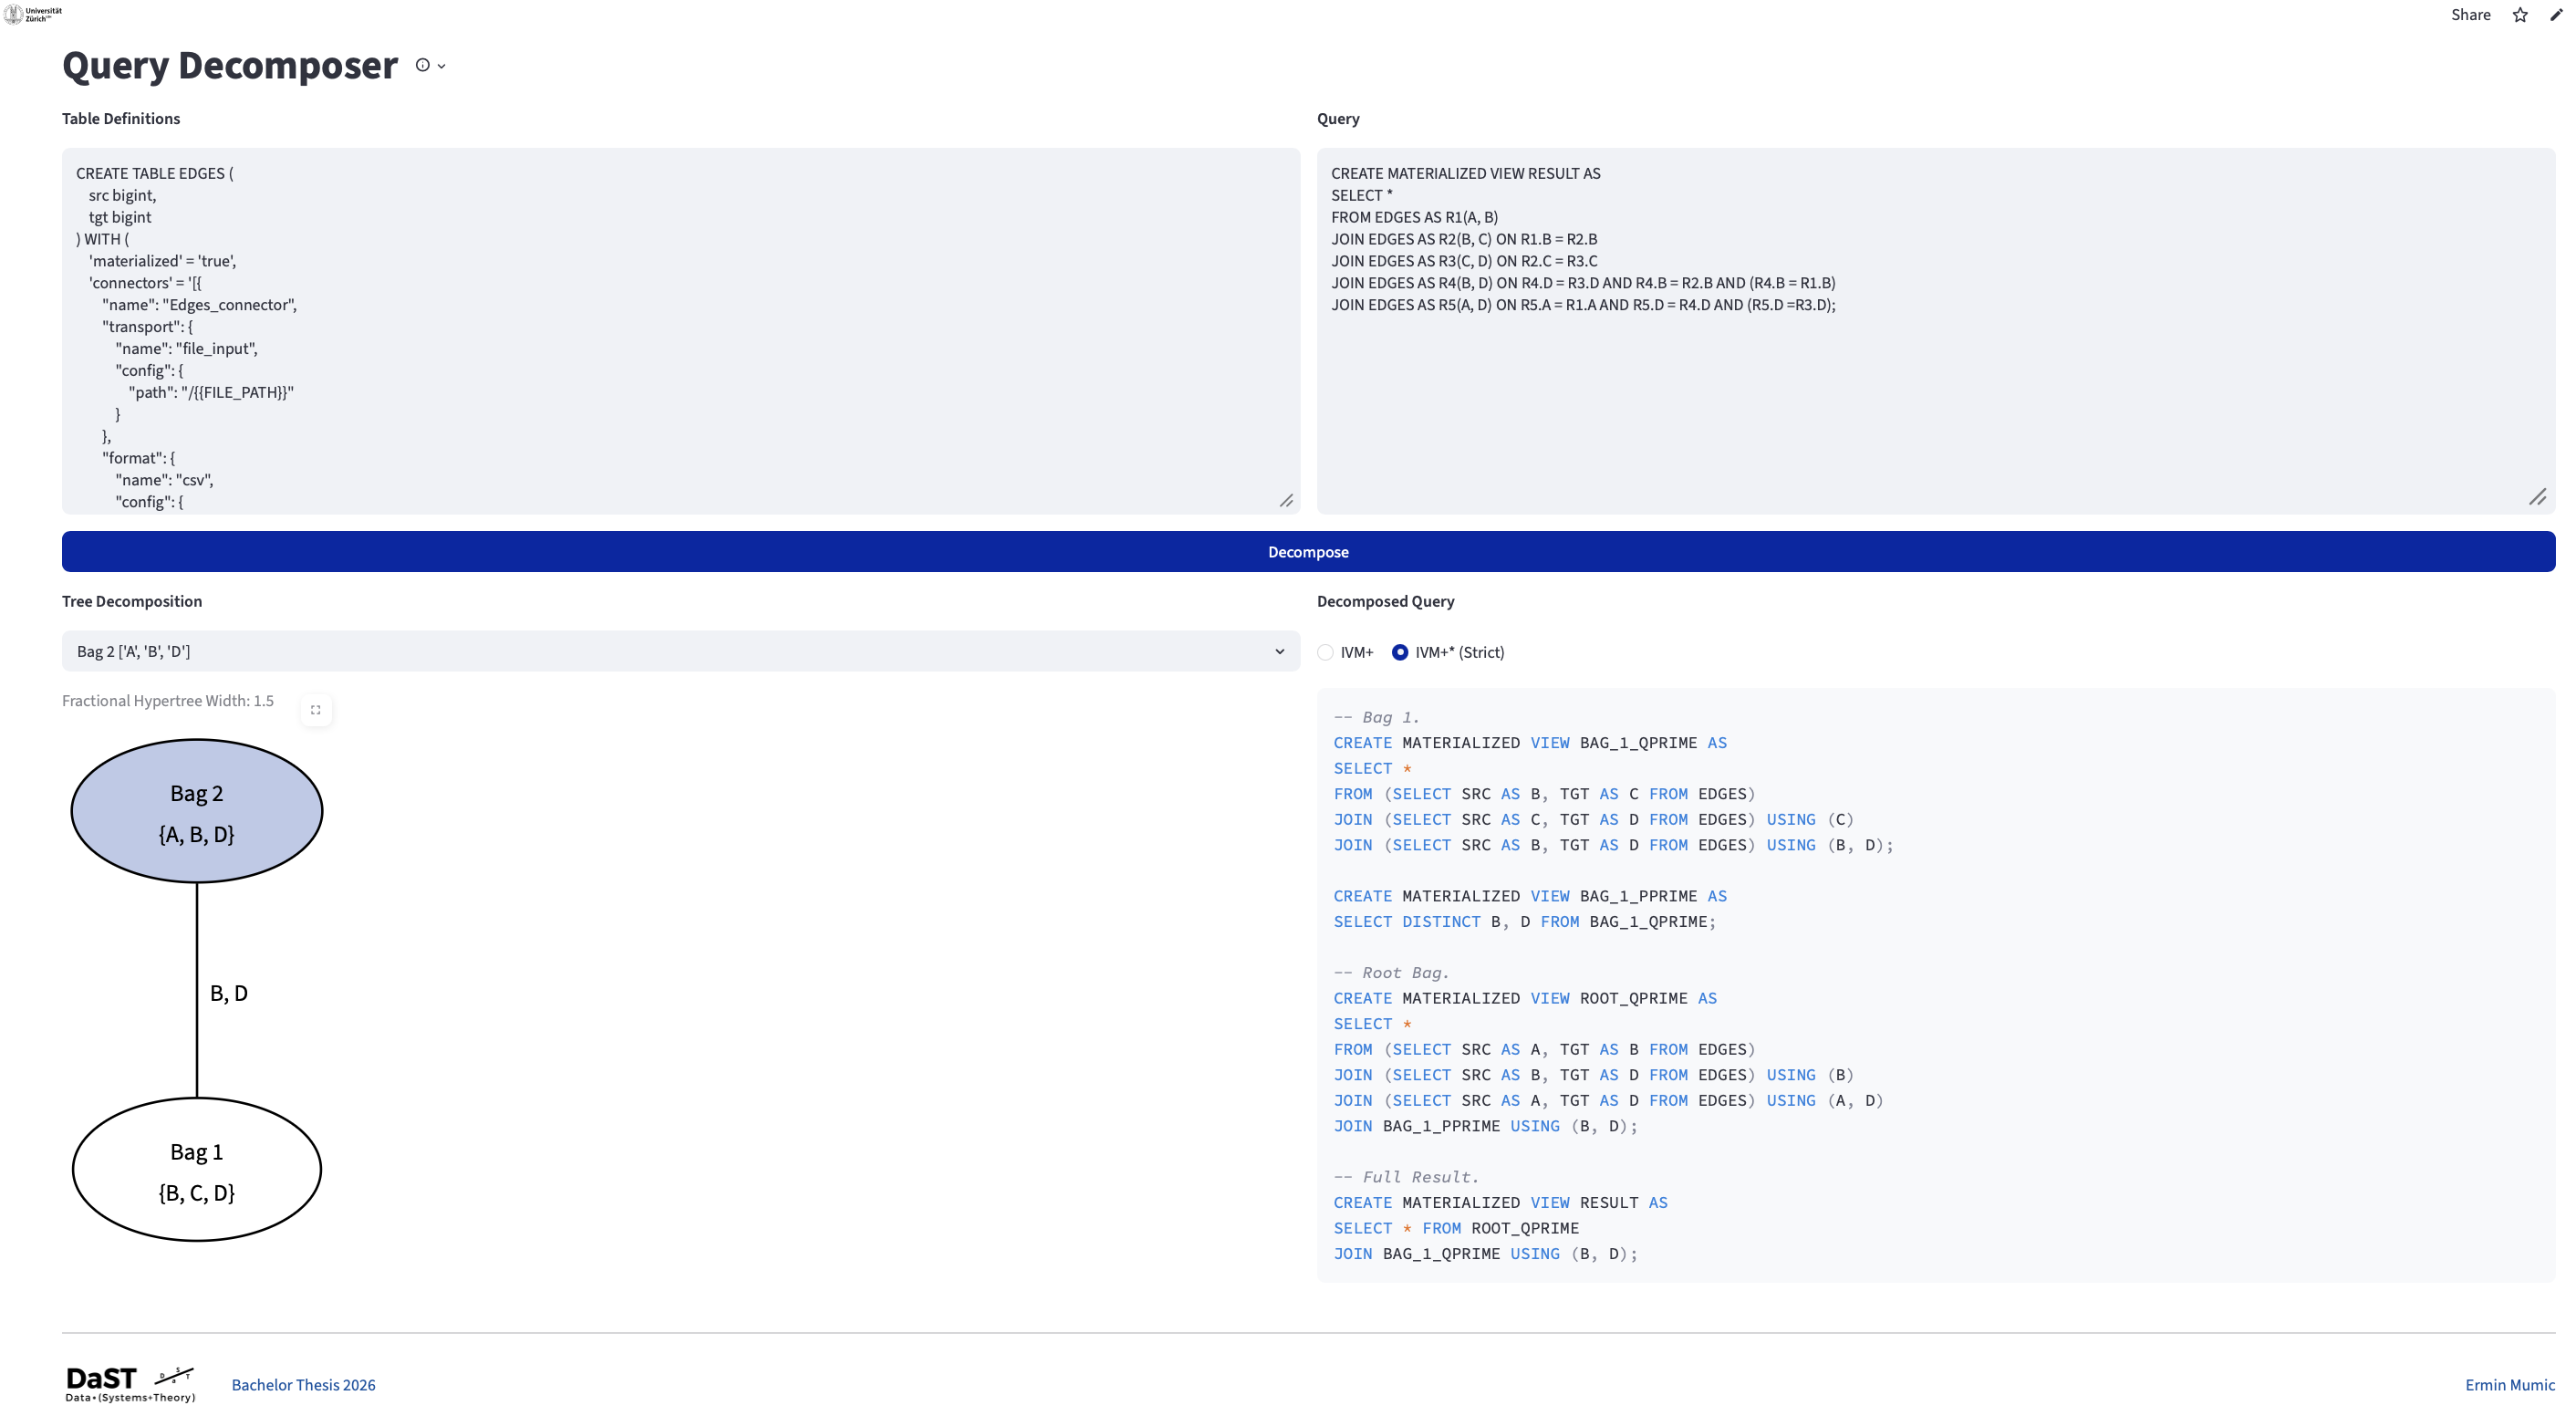
\includegraphics[width=\textwidth]{./figures/ch4_web_ui.png}
  \caption{The query decomposer's web interface on $Q_\diamond$.}
  \label{fig:decomposer_ui}
\end{figure}

These views are the artifact the experiment harness deploys.

\subsection{Supported queries and limitations}
\label{sec:decomposer_limits}

The decomposer handles \emph{full conjunctive queries} over an input schema, the class the IVM$^+$ approach targets.
The schema is given as \texttt{CREATE TABLE} statements, of which the parser reads only the column definitions and ignores the rest, so the Feldera-specific connector and materialisation annotations of Section~\ref{sec:pipeline} may be left in place and the same schema used for a pipeline can be handed to the decomposer unchanged.

A query must be a single \texttt{SELECT *} or \texttt{SELECT COUNT(*)}.
In both cases the decomposer emits the bag views and a final \texttt{RESULT} view.
For \texttt{SELECT *} the \texttt{RESULT} view reconstructs the full join, and for \texttt{SELECT COUNT(*)} it returns the count, computed on the decomposition by the semiring aggregate of Section~\ref{sec:pipeline}.
Tables and columns may be aliased, and a relation may occur several times, so self-joins such as $Q_\diamond$ are supported, written either \texttt{EDGES AS R1} or with a renamed column list \texttt{EDGES AS R1(A, B)}.
Joins must be equi-joins, written \texttt{JOIN \ldots ON $c_1$ = $c_2$} or \texttt{JOIN \ldots USING}.
The \texttt{WHERE} clause may carry filters that each reference a single relation, combined with \texttt{AND}, and each such filter is pushed into that relation's subquery.

\medskip

Everything outside this class is rejected or unsupported.
\texttt{COUNT(*)} is the only aggregate, and other aggregates and projections of specific columns are not available.
Only equi-joins are recognised, so inequality and outer joins are not supported.
A \texttt{WHERE} condition that spans more than one relation is rejected, whether a comparison between columns of different relations or a disjunction across them.
A filter on each relation separately, joined by \texttt{AND}, is the supported form.
Subqueries are not supported.

Finally, the decomposer performs only the checks its translation needs and is not a full SQL validator.
A query should therefore be validated in a database engine, for instance Feldera itself, before it is given to the decomposer.

\bigskip

In this chapter, we detail the implementation of the components required to evaluate the theoretical IVM$^+$ approach in practice. This includes the manual translation of tree decompositions into Feldera SQL pipelines, as well as the development of an automated, multi-threaded benchmarking harness designed to orchestrate the experiments.
\paragraph{Materialization policy.}
Feldera materializes a relation only when explicitly requested, and materializes a
base table automatically when a \texttt{PRIMARY KEY} is declared, since it must
maintain a key index. Materialization additionally stores a relation's full
contents so it can be queried at runtime; it is a storage feature rather than a
performance optimization. To keep the comparison fair, we hold materialization
identical across all variants except for the single view whose output each
experiment reads. All base tables use the same schema in every variant, so any
storage they incur (for example, from primary keys) is constant across the
baseline and the IVM$^+$ configurations and cancels out of the comparison. Among
the derived views we materialize only the terminal view that an experiment
measures --- the reconstructed \texttt{RESULT} for the baseline and the rejoining
variant, and the root bag for the non-rejoining variant --- and leave all
intermediate bag views non-materialized. We keep the terminal view materialized so
that Feldera does not prune the computation that feeds it.

final result reconstruction throug:In practice, this is expressed as a final SQL view that joins all bag Q-views along the bridge columns.

\section{IVM$^+$ Translation and Pipeline Construction}
\label{sec:manual_translation}

Each experimental query variant is expressed as a self-contained Feldera SQL file that defines both the input schema with its data connectors and the sequence of materialized views encoding the query logic. All files are parameterized templates: the literal \texttt{\{\{FILE\_PATH\}\}} is substituted at runtime by the benchmarking harness (see Section~\ref{sec:benchmark_harness}) with the actual dataset path, allowing the same pipeline definition to run against multiple datasets without modification, provided they conform to the same relational schema (e.g., executing the same TPC-H query template across Scale Factors 1, 10, and 30).

\subsection{IVM$^+$ Decomposition Translation}
\label{sec:decomposition_translation}

The IVM$^+$ algorithm (see Chapter~\ref{ch:ivm}) operates on a tree decomposition of the query hypergraph. Each node of the decomposition tree is a \emph{bag} that groups a subset of the query relations. Translating this structure into Feldera SQL, every bag is represented by a pair of materialized views, which instruct the DBSP engine to physically store and incrementally update the view's contents after every insert.:

\begin{itemize}
    \item \textbf{Q-view} (\texttt{CHILD\_N\_Q}, \texttt{ROOT\_Q}): corresponding to the $Q'$-relation in the theoretical formulation.
    \item \textbf{P-view} (\texttt{CHILD\_N\_P}): computed as \texttt{SELECT DISTINCT} over the join attributes. This corresponds to the $P'$-relation.
\end{itemize}

Views are defined bottom-up following the tree structure, so each child's P-view is available when the parent's Q-view is computed. The final \texttt{RESULT} view reconstructs the full output by joining all Q-views back together.

For multi-relation schemas, we use \texttt{JOIN \ldots USING} rather than explicit \texttt{ON} conditions. SQL's \texttt{JOIN USING} guarantees that the named join column appears only once in the output, making \texttt{SELECT *} unambiguous regardless of how many Q-views are chained together. For graph queries, where all relations share the same underlying \texttt{(src, tgt)} schema, each Q-view aliases its columns explicitly (e.g.\ \texttt{R1.A AS A, R1.B AS B}), and joins use explicit \texttt{ON} conditions instead.

In addition to the full-join decomposition variants, we also implemented FAQ (Functional Aggregate Query) variants that compute an aggregate directly over the decomposition using a semiring, rather than materializing the full join result. These are discussed and evaluated in Chapter~\ref{ch:evaluation}.

\subsection{Input Connectors}
\label{sec:input_connectors}

Feldera ingests data through connector annotations attached to \texttt{CREATE TABLE} declarations. We use the built-in \texttt{file\_input} connector with the CSV format. Two connector patterns appear across the pipelines, depending on the dataset.

For multi-relation schemas such as TPC-H and IMDB, each table points to its own CSV file within the dataset directory:

\begin{lstlisting}[caption={Per-table CSV connector for multi-relation datasets (TPC-H).}]
CREATE TABLE ORDERS (
    ORDERKEY bigint not null,
    CUSTKEY  bigint not null,
    ...
    PRIMARY KEY (ORDERKEY)
) WITH (
    'connectors' = '[{
        "transport": {
            "name": "file_input",
            "config": { "path": "/{{FILE_PATH}}/orders.csv" }
        },
        "format": { "name": "csv", "config": { "headers": true } }
    }]'
);
\end{lstlisting}

For homogeneous graph datasets (SNAP), all relations share the same edge schema. Two sub-variants exist here. In the \emph{single-table} variant, one \texttt{EDGES} table is declared with a single connector and then aliased at the query level with renamed columns (e.g.\ \texttt{EDGES AS R1(A, B)}). In the \emph{multi-table} variant, each logical relation $R_1, R_2, \ldots$ is declared as a separate table, each with its own connector pointing to the same CSV file. The multi-table form matches the theoretical schema more directly and avoids SQL aliasing, at the cost of loading the edge file once per relation. The performance implications of both strategies are discussed in Chapter~\ref{ch:evaluation}.

\begin{lstlisting}[caption={Single-file CSV connector for graph datasets.}]
CREATE TABLE EDGES (
    src bigint,
    tgt bigint
) WITH (
    'materialized' = 'true',
    'connectors' = '[{
        "transport": {
            "name": "file_input",
            "config": { "path": "/{{FILE_PATH}}" }
        },
        "format": { "name": "csv", "config": { "headers": true } }
    }]'
);
\end{lstlisting}

All tables in the dataset schema are always declared, even those not directly queried. Tables not participating in the query are declared without a connector (annotated \texttt{'materialized' = 'true'} only), which registers their column types in Feldera's catalog but causes no data to be ingested into them.

\subsection{Pipeline Variants}
\label{sec:pipeline_variants}

We implemented three core pipeline types for each query. Each is a self-contained Feldera SQL file.

\subsubsection{Baseline}
\label{sec:baseline_pipelines}

The baseline expresses the original query as a single flat join without any tree decomposition, serving as the non-IVM$^+$ reference point for the evaluation. The following example shows the 3-table TPC-H path query:

\begin{lstlisting}[caption={Baseline 3-table TPC-H path query.}]
CREATE MATERIALIZED VIEW RESULT AS
SELECT *
FROM LINEITEM
JOIN SUPPLIER USING (SUPPKEY)
JOIN CUSTOMER USING (NATIONKEY);
\end{lstlisting}

\subsubsection{IVM$^+$ Decomposition}
\label{sec:decomp_standard}

The IVM$^+$ decomposition follows the $Q'$-relation definition from Chapter~\ref{ch:ivm}: the Q-view for each bag is the restriction $Q[\chi(t)]$ of the full query to the bag's variables, with partial atoms projected to their shared variables as inline \texttt{JOIN (SELECT DISTINCT \ldots) USING (\ldots)} semijoins, and joined with the $P'$-views of any child bags. The following example shows the 3-table TPC-H path query, where \texttt{LINEITEM} and \texttt{CUSTOMER} are children of a root bag containing \texttt{SUPPLIER}:

\begin{lstlisting}[caption={IVM$^+$ decomposition (3-table TPC-H).}]
-- Child Bag 1: Q[chi(1)] -- LINEITEM with partial atoms projected.
CREATE MATERIALIZED VIEW CHILD_1_Q AS
SELECT * FROM LINEITEM
JOIN (SELECT DISTINCT SUPPKEY FROM SUPPLIER) USING (SUPPKEY);

CREATE MATERIALIZED VIEW CHILD_1_P AS
SELECT DISTINCT SUPPKEY FROM CHILD_1_Q;

-- Child Bag 2: Q[chi(2)] -- CUSTOMER with partial atoms projected.
CREATE MATERIALIZED VIEW CHILD_2_Q AS
SELECT * FROM CUSTOMER
JOIN (SELECT DISTINCT NATIONKEY FROM SUPPLIER) USING (NATIONKEY);

CREATE MATERIALIZED VIEW CHILD_2_P AS
SELECT DISTINCT NATIONKEY FROM CHILD_2_Q;

-- Root Bag: Q[chi(root)] joined with children's P-views.
CREATE MATERIALIZED VIEW ROOT_Q AS
SELECT *
FROM SUPPLIER
JOIN (SELECT DISTINCT SUPPKEY   FROM LINEITEM) USING (SUPPKEY)
JOIN (SELECT DISTINCT NATIONKEY FROM CUSTOMER) USING (NATIONKEY)
JOIN CHILD_1_P USING (SUPPKEY)
JOIN CHILD_2_P USING (NATIONKEY);

-- Result: full output reconstructed from all Q-views.
CREATE MATERIALIZED VIEW RESULT AS
SELECT *
FROM ROOT_Q
JOIN CHILD_1_Q USING (SUPPKEY)
JOIN CHILD_2_Q USING (NATIONKEY);
\end{lstlisting}

These pipelines are annotated \texttt{decomposition\_full} in the pipeline files.

\subsubsection{IVM$^+$ Decomposition Without Semijoin}
\label{sec:decomp_no_semijoin}

This variant uses the adjusted $Q^*$-relation definition from Chapter~\ref{ch:ivm}: only atoms whose variable set contains all bag variables ($\chi(t) \subseteq \mathbf{X}_i$) are included in a bag's Q-view. Atoms with partial overlap are dropped rather than projected. All bags with children are still joined with those children's $P'$-views in the bottom-up computation. These pipelines are annotated \texttt{decomposition\_no\_projection\_full} in the pipeline files.

\paragraph{Restriction to graph datasets.}
For the homogeneous graph queries, every atom is an instance of the same \texttt{EDGES} relation. An inline semijoin in a bag therefore reduces to filtering that bag by the set of nodes appearing on a single endpoint of the edge relation, i.e.\ $\pi_{\text{src}}\,E$ or $\pi_{\text{tgt}}\,E$. The elimination of dangling tuples that the decomposition relies on is already performed bottom-up by the children's $P'$-relations; the additional single-endpoint projections cover most nodes in the densely connected graphs we study, so they remove few tuples while still incurring the cost of maintaining the extra \texttt{SELECT DISTINCT} and join operators. For this reason we restrict the graph experiments to the without-semijoin variant ($Q^*$). The projection (semijoin) variant is evaluated only on the multi-relation TPC-H and IMDB datasets, where the atoms are distinct relations and the inline projections act as genuine filters.

\begin{lstlisting}[caption={IVM$^+$ decomposition without semijoin (3-table TPC-H).}]
-- Child Bag 1: Q*(chi(1)) = LINEITEM (chi(1) subset X_LINEITEM).
CREATE MATERIALIZED VIEW CHILD_1_Q AS
SELECT * FROM LINEITEM;

CREATE MATERIALIZED VIEW CHILD_1_P AS
SELECT DISTINCT SUPPKEY FROM CHILD_1_Q;

-- Child Bag 2: Q*(chi(2)) = CUSTOMER (chi(2) subset X_CUSTOMER).
CREATE MATERIALIZED VIEW CHILD_2_Q AS
SELECT * FROM CUSTOMER;

CREATE MATERIALIZED VIEW CHILD_2_P AS
SELECT DISTINCT NATIONKEY FROM CHILD_2_Q;

-- Root Bag: Q*(chi(root)) joined with children's P-views.
CREATE MATERIALIZED VIEW ROOT_Q AS
SELECT *
FROM SUPPLIER
JOIN CHILD_1_P USING (SUPPKEY)
JOIN CHILD_2_P USING (NATIONKEY);

-- Result: full output reconstructed from all Q-views.
CREATE MATERIALIZED VIEW RESULT AS
SELECT *
FROM ROOT_Q
JOIN CHILD_1_Q USING (SUPPKEY)
JOIN CHILD_2_Q USING (NATIONKEY);
\end{lstlisting}

\subsection{Further Variants}
\label{sec:further_variants}

The three core pipeline types above were each extended along the following dimensions.

\subsubsection{Input Connector Variants}
\label{sec:connector_variants}

All pipeline types --- including the baseline --- come in two connector sub-variants for homogeneous graph datasets (SNAP): a \emph{single-table} variant using one \texttt{EDGES} table with SQL aliasing, and a \emph{multi-table} variant with a separate table declaration per relation. Both sub-variants are described in Section~\ref{sec:input_connectors}; multi-relation datasets (TPC-H, IMDB) are unaffected as each table already has its own connector.

\subsubsection{Root Orientation}
\label{sec:decomp_root}

Where the decomposition admits more than one root, both decomposition variants were evaluated under two different root orientations of the tree decomposition, labelled \textbf{D1} and \textbf{D2} in the result tables of Chapter~\ref{ch:evaluation}. A tree decomposition does not prescribe a canonical root; choosing a different bag as root changes which bag aggregates last and therefore which intermediate views grow largest. The \texttt{chain\_decomposition} pipeline files correspond to one orientation (\textbf{D1}), \texttt{decomposition} to the other (\textbf{D2}). Not every query admits two meaningfully distinct orientations, however: when the decomposition is trivial --- for instance when it consists of only two bags, or when its shape is symmetric under re-rooting --- the two orientations coincide, and only a single orientation (\textbf{D1}) is reported for that query. The specific root choice and its performance implications for each query are discussed in Chapter~\ref{ch:evaluation}.

\subsubsection{Without Result Reconstruction}
\label{sec:no_reconstruction}

For both decomposition variants, a version exists that omits the final \texttt{RESULT} reconstruction join: \texttt{ROOT\_Q} is exposed directly as \texttt{RESULT}, containing only the root bag's columns. These pipelines (annotated without the \texttt{\_full} suffix) isolate the cost of maintaining the Q- and P-view hierarchy from the cost of joining all bags back together for the full output.

\subsubsection{FAQ Variant}
\label{sec:faq_variant}

Building on the without-reconstruction pipelines, the FAQ (Functional Aggregate Query) variant replaces the final result with a semiring-based aggregate computed directly over the decomposition, rather than materialising the full join output. Both decomposition types have a corresponding FAQ variant, annotated \texttt{\_faq} in the pipeline files. A detailed discussion of the semiring formulation and its performance implications is deferred to Chapter~\ref{ch:evaluation}.

\section{Automated Benchmark Harness}
\label{sec:benchmark_harness}

To reliably orchestrate the experiments, guarantee reproducible environments and capture precise system metrics, we developed a benchmarking framework in Python. The Feldera engine itself is deployed within a Docker container on a dedicated remote machine. Our framework, consisting of a top-level automation orchestrator (\texttt{automation.py}) and a core execution script (\texttt{experiment.py}), runs directly on this same remote host, interacting with the containerized engine locally via its REST API using the Feldera Python SDK wrapper.

\subsection{Automation Orchestrator}
Evaluating database engines requires isolation to ensure that residual memory caches or disk states from previous queries do not interfere with subsequent benchmarks. To achieve this, the overarching Automation Orchestrator enforces a strict "cold start" for every query variant in the experimental queue.

Prior to execution, the orchestrator uses system-level commands to shut down the local Feldera Docker containers (\texttt{docker compose down -v}) and forcefully prune the Docker system. Crucially, we mapped the container's primary working directory to a physical volume on the host machine (\texttt{/local/scratch/emumic/feldera\_storage}) to accommodate the massive intermediate views required by IVM$^+$. During the cold start phase, the orchestrator completely wipes this host directory. Since Docker creates this directory as root, it cannot be deleted directly from the host without elevated privileges. To bypass this, the orchestrator spawns a temporary Ubuntu container with the host path bind-mounted and deletes the directory from within that container as root. The directory is then recreated with open permissions before the engine is restarted.

The Docker containers are then rebuilt and given a 30-second initialization buffer, guaranteeing that every experiment begins with zero cached data. To manage the extensive suite of benchmarks safely, the orchestrator wraps the entire pipeline execution in a global 15-hour timeout threshold. Upon completion, timeout or crash, it logs the final status and duration to a global overview file before proceeding to the next configuration.

\subsection{Execution Script}
Once the orchestrator has prepared a clean environment, it triggers the core benchmarking script (\texttt{experiment.py}). To allow the containerized Feldera engine to access the host's local datasets without network overhead, the data directory on the remote machine is mounted as a volume directly into the Docker container. 

To monitor these dataflow pipelines without interrupting the main execution flow, the script utilizes a multi-threaded architecture based on Python's native \texttt{threading} module:

\begin{itemize}
    \item \textbf{Task Workers (Blocking Execution):} We implemented a generic \texttt{TaskWorker} thread class to handle synchronous operations. Once the pipeline starts, a task worker is spawned to wait for the process to complete. To prevent infinite hangs, this thread is joined with a strict three-hour timeout constraint. A secondary task worker handles the final result-count query (with a one-hour timeout) to verify computational correctness.
    
    \item \textbf{Stats Poller (Asynchronous Monitoring):} Concurrent to the primary task worker, a \texttt{StatsPoller} daemon thread continuously queries Feldera's \texttt{/stats} API endpoint. The poller captures the pipeline's uptime, total completed records and Resident Set Size (RSS) memory footprint. The polling interval is strictly configured to 5 seconds. This thread is terminated via a threading event once the primary task worker successfully joins or times out.
\end{itemize}

Upon pipeline termination, the harness aggregates the chronological timeline of polled metrics, calculates the global throughput (rows per second), extracts the peak memory consumption and serializes the complete payload into a JSON artifact for later analysis. To isolate individual trials within the same experiment run, the harness additionally calls \texttt{pipeline.clear\_storage()} after each trial, wiping Feldera's internal incremental state so that the next trial begins from a clean state without requiring a full Docker restart.

\section{Automated Query Parser}
\label{sec:query_parser}
